\documentclass[t]{beamer}

%\documentclass[handout, t]{beamer}
\setbeamertemplate{navigation symbols}{}
\usepackage{pstricks}
\usepackage{mathtools}
\usepackage{amsfonts}
\usepackage{mathrsfs}
\usepackage{amsmath}
\setbeamertemplate{navigation symbols}{}
\usepackage{bm}
\usepackage[UTF8]{ctex}
\usetheme{AnnArbor}
\usefonttheme{serif}
\useinnertheme{rounded}
%\usecolortheme{crane}
\setbeamertemplate{blocks}[rounded][shadow=true]

\newcommand{\dif}{{\;\rm d}}
\usepackage{graphicx}
\usepackage{pgf}
\usepackage{tikz}
\usetikzlibrary{arrows, decorations.pathmorphing, backgrounds, positioning, fit, petri, automata}
\tikzset{>=stealth}

\usepackage{setspace}
\setmainfont{Times New Roman}
\setCJKmainfont{Microsoft YaHei}
\usepackage{physics}

\hypersetup{pdfpagemode=FullScreen}
\renewcommand{\Pr}{\mathbb{P}}
\usepackage{blkarray}


\setbeamercolor{block title}{bg=red!10!white}
\setbeamercolor{block body}{bg=gray!10!white}

\usepackage{multicol}
\newcommand{\E}{\mathbb{E}}
\newcommand{\EP}{\mathbb{E}^{\mathbb{P}}}
\newcommand{\EQ}{\mathbb{E}^{\mathbb{Q}}}
\newcommand{\Var}{{\rm Var}}
\newcommand{\Cov}{{\rm Cov}}


\begin{document}
\fontsize{11}{18}\selectfont


\CTEXindent



  \title{第四章~~泊松过程}
\author{随机过程及其在金融中的应用}
\date{中国人民大学出版社}
  \begin{frame}
    \maketitle
  \end{frame}

\begin{frame}{本章内容}
  \begin{multicols}{2}
    \tableofcontents
  \end{multicols}
\end{frame}

\begin{frame}{引言}
    泊松过程(Poisson process)是一类重要的时间连续、状态离散的随机过程。作为以法国数学家泊松(Simeon Denis Poisson)命名的随机过程,这是一类非常特殊的计数过程(counting process),由于其良好的性质,在很多学科领域均有应用,比如:信号处理、金融工程、风险管理、运筹学等。
    
\begin{center}
\includegraphics[height=.45\textheight]{fig/poisson.jpg}
\end{center}

\end{frame}


\section{指数分布}
\subsection{指数分布的基本概念}

\begin{frame}{指数分布的基本概念}
    若随机变量$T$满足
\begin{equation*}
\Pr(T\le t)=1-{\rm e}^{-\lambda t},\qquad \forall t\ge 0
\end{equation*}
则称其服从速率为$\lambda$的指数分布(exponential distribution),记作$T\sim \mathcal{E}(\lambda)$。

记$F(t)=\Pr(T\le t)$为分布函数,则相应的密度函数如下:
\[f_T(t)=\begin{cases}
\lambda {\rm e}^{-\lambda t},& t\ge 0\\
0,& t<0
\end{cases} \]
\end{frame}

\subsection{指数分布的矩}
\begin{frame}{指数分布的矩}
    \begin{enumerate}
        \item 	一阶矩(期望):
            \[\E(T)=\int^{\infty}_0 t\cdot f_T(t)\dif t=\int_{0}^{\infty}t\cdot \lambda {\rm e}^{-\lambda t}\dif t=\frac{1}{\lambda}
            \]
        \item 二阶矩:
        \[\E(T^2)=\int^{\infty}_0 t^2\cdot f_T(t)\dif t=\int_{0}^{\infty}t^2\cdot \lambda {\rm e}^{-\lambda t}\dif t=\frac{2}{\lambda^2}\]	
        \item 方差:
        \[{\rm Var}(T)= \E(T^2)-[\E(T)]^2=\frac{2}{\lambda^2}-\frac{1}{\lambda^2}=\frac{1}{\lambda^2}\]
        \end{enumerate}
\end{frame}


\begin{frame}{指数分布的矩(cont.)}
    对于$T\sim\mathcal{E}(\lambda)$,其均值为$1/\lambda$,方差为$1/\lambda^2$。
    
    若$S=\lambda T$,则
$S\sim\mathcal{E}(1)$,其均值为$1$,方差也为$1$。

\begin{block}{简要证明:}
	由于$T\sim\mathcal{E}(\lambda)$,$S\sim\mathcal{E}(1)$,假设$Z=S/\lambda$,则对$\forall\; t$,有:
	\[\begin{split}
	\Pr(Z\le t)&=\Pr(S/\lambda\le t)=\Pr(S\le \lambda t)\\
	&=1-\exp\left[-1\cdot (\lambda t)\right]=1-{\rm e}^{-\lambda t}\\
	&=\Pr(T\le t)
	\end{split}\quad \Rightarrow \quad T=Z=\frac{S}{\lambda}\]
\end{block}
\end{frame}

\subsection{指数分布的性质}
\begin{frame}{指数分布的无记忆性}
    假设$T$服从速率为$\lambda$的指数分布,则:
\begin{equation*}
	{\Pr(T>t+s|T>t)}={\Pr(T>s)} 
\end{equation*}

\begin{block}{简要证明:}
    由于:
    \[\Pr(T\le t)=1-{\rm e}^{-\lambda t}\quad\Rightarrow\quad \Pr(T>t)={\rm e}^{-\lambda t} \]	
    因此:
    \[\begin{split}
    {\Pr(T>t+s|T>t)}&=\frac{\Pr(T>t+s,\;T>t)}{\Pr(T>t)}\\
    &=\frac{\Pr(T>t+s)}{\Pr(T>t)}=\frac{{\rm e}^{-\lambda(t+s)}}{{\rm e}^{-\lambda t}}={\rm e}^{-\lambda s}={\Pr(T>s)}
    \end{split}\]
\end{block}

\end{frame}


\begin{frame}{指数分布的无记忆性(cont.)}
    \[	{\Pr(T>t+s|T>t)}={\Pr(T>s)} 
    \]

    如果将$T$看作一个仪器的寿命,那么上式说明了,在该仪器已经正常工作$t$小时的前提下,其继续正常工作$s$小时的(条件)概率,与其出厂后正常工作$s$小时的(无条件)概率是完全相等的。也就是说,仪器之前正常工作的$t$小时,不会对其未来正常工作的时间产生任何影响,该特征就是无记忆性(lack of memory)。
    
    \begin{block}{注意:}
指数分布是唯一具有无记忆性的连续型概率分布。
    \end{block}
   
\end{frame}


\begin{frame}{举例}
    假设顾客在银行的时间服从均值为10分钟的指数分布,问:
\begin{enumerate}
\item 一个顾客在此银行用时超过15分钟的概率是多少?
\item 假定一个顾客10分钟后仍在银行,则她在银行用时超过15分钟的概率是多少?
\end{enumerate}

\begin{block}{注意:}
   此处 $\lambda=1/10$。
\end{block}

\end{frame}


\begin{frame}{解答}
    
如果以$X$表示顾客在这个银行的时间,则问题(1)中的概率如下:
\[\Pr(X> 15)={\rm e}^{-\lambda t}=\exp\qty(-\frac{1}{10}\times 15)=0.22 \]

问题(2)需要求一个已经在银行用时10分钟的顾客至少再用时5分钟的概率。
根据指数分布的无记忆性,该概率与之前的用时无关,且等于
一个刚进入银行的顾客停留至少5分钟的概率,即要求的概率如下:
\[\Pr(X> 5)={\rm e}^{-\lambda t}=\exp\qty(-\frac{1}{10}\times 5)=0.604 \]
\end{frame}



\begin{frame}{定理1}\small
    假设$T_i$服从速率为$\lambda_i$的指数分布$(i=1,2,\ldots,n)$,且$T_i$之间相互独立。则:
\begin{equation*}
	\min(T_1,T_2,\ldots,T_n)\sim \mathcal{E}(\lambda_1+\lambda_2+\cdots+\lambda_n)
\end{equation*}
\begin{block}{简单证明}
    由不等式的性质,可得:	
	\[\begin{split}
	{\Pr[\min(T_1,T_2,\ldots,T_n)>t]}&=\Pr(T_1>t,T_2>t,\ldots, T_n>t)\\
	&=\prod_{i=1}^{n}\Pr(T_i>t)=\prod_{i=1}^{n}{\rm e}^{-\lambda_i t}\\
	&={\exp\left[-(\lambda_1+\lambda_2+\cdots+\lambda_n)t \right]}
	\end{split}
	\]
	即:$$\min(T_1,T_2,\ldots,T_n)\sim \mathcal{E}(\lambda_1+\lambda_2+\cdots+\lambda_n)$$
\end{block}

\end{frame}


\begin{frame}{定理2}\small
    假设$T_1\sim \mathcal{E}(\lambda_1)$,$T_2\sim \mathcal{E}(\lambda_2)$,且两者相互独立,则:
\begin{equation*}
\E\left[\max(T_1,T_2) \right]=\frac{1}{\lambda_1}+\frac{1}{\lambda_2}-\frac{1}{\lambda_1+\lambda_2}
\end{equation*}
\begin{block}{简单证明}
由下列恒等式:
	$$\max(T_1,T_2)=T_1+T_2-\min(T_1,T_2)$$
	根据期望的线性性质,可得:
	\[\begin{split}
	\E[\max(T_1,T_2)]&=\E( T_1)+\E( T_2)-\E[\min(T_1,T_2)]\\
	&=\frac{1}{\lambda_1}+\frac{1}{\lambda_2}-\frac{1}{\lambda_1+\lambda_2}
	\end{split} \]
\end{block}
\end{frame}

\begin{frame}{定理3:指数分布的排序}
    \small
    假设$T_1\sim \mathcal{E}(\lambda_1)$,$T_2\sim \mathcal{E}(\lambda_2)$,且两者相互独立 ,则:
    \begin{equation*}
    \Pr(T_1<T_2)=\Pr[T_1=\min(T_1,T_2)]=\frac{\lambda_1}{\lambda_1+\lambda_2}
\end{equation*}

\begin{block}{简单证明}
        利用卷积公式,证明如下:
\[\begin{split}
\Pr(T_1<T_2)&=\int^{\infty}_0 f_{T_1}(u)\Pr(u<T_2)\dif u
=\int^{\infty}_0 \lambda_1{\rm e}^{-\lambda_1 u}{\rm e}^{-\lambda_2 u}\dif u\\
&=\int^{\infty}_0 \lambda_1 {\rm e}^{-(\lambda_1+\lambda_2)u}\dif u=\frac{\lambda_1}{\lambda_1+\lambda_2}
\end{split}\]
        \end{block}
\end{frame}


\begin{frame}{推论}
    $T_i$是$T_1,T_2,\ldots,T_n$中最小随机变量的概率为:
	\begin{equation*}
	\Pr[T_i=\min(T_1,T_2,\ldots,T_n)]=\frac{\lambda_i}{\lambda_1+\lambda_2+\cdots+\lambda_n},\qquad i=1,2,\ldots,n
	\end{equation*} 

    
\end{frame}


\begin{frame}{举例1}
    假设小明到达邮局时,邮局的两位办事员都在忙,并且没有人在排队等待。只要有一位办事员有空,就可以为小明提供服务。假设办事员$i$的服务时间服从速率为$\lambda_i$的
指数分布($i=1,2$),求小明待在邮局的期望时间。

\begin{block}{思路:}
    小明待在邮局的时间分成两段:一段是等待两位办事员中的一位忙完所需要的时间,记作$W$;另一段是其中一位办事员为小明提供服务所需的时间,记作$S$。
于是问题就转化成求$\E(W)+\E(S)$。进一步假设两位办事员完成当前工作所需的时间分别为$T_1$和$T_2$。
\end{block}
\end{frame}


\begin{frame}{举例1(cont.)}
    首先,小明等待的时间$\E(W)$应当为$T_1$和$T_2$之中的较小值,于是有:
\[\E(W)=\E[\min(T_1,T_2)]=\frac{1}{\lambda_1+\lambda_2} \]

接下来,如果是办事员1先结束当前业务,其对应的概率为:
\[\Pr(T_1<T_2)=\frac{\lambda_1}{\lambda_1+\lambda_2} \]
在此情形下,由办事员1为小明提供服务,相应的服务时间期望值为$1/\lambda_1$;
类似地,如果是办事员2先结束当前服务,其对应的概率为:
\[\Pr(T_1>T_2)=\frac{\lambda_2}{\lambda_1+\lambda_2} \]
在此情形下,由办事员2为小明提供服务,相应的服务时间期望值为$1/\lambda_2$。
\end{frame}


\begin{frame}{举例1(cont.)}
    将两种情形综合起来,可得:
\[\begin{split}
\E(S)&=\E(T_1)\cdot \Pr(T_1<T_2)+\E(T_2)\cdot \Pr(T_1>T_2)\\
&=\frac{1}{\lambda_1}\cdot \frac{\lambda_1}{\lambda_1+\lambda_2}+\frac{1}{\lambda_2}\cdot \frac{\lambda_2}{\lambda_1+\lambda_2}\\
&=\frac{2}{\lambda_1+\lambda_2}
\end{split}
\]
最终可得:
\[\E(W)+\E(S)=\frac{3}{\lambda_1+\lambda_2} \]
\end{frame}



\begin{frame}{举例2}
    C进入一家邮局,发现A和B分别在接受办事员1和办事员2的服务。已知两位办事员服务的时间服从速率为$\lambda_i$的指数分布($i=1,2$)
	。
	
    问:C最后一个离开邮局的概率是多少?
    

\end{frame}


\begin{frame}{举例2:方法一}
    假设A和B二人当中,A先办完事情离开,相应的概率为${\lambda_1}/{(\lambda_1+\lambda_2)}$。
此时只剩下C和B在邮局办理业务。根据指数分布的无记忆性,接下来B先办完事情离开的概率为
${\lambda_2}/{(\lambda_1+\lambda_2)} $。

类似地,B先办完事情离开的概率为${\lambda_2}/{(\lambda_1+\lambda_2)}$。
此时只剩下A和C在邮局办理业务。根据指数分布的无记忆性,接下来A先办完事情离开的概率为${\lambda_1}/{(\lambda_1+\lambda_2)}$。

因此,将两种情形下的概率相加,最终可得:
\[\frac{\lambda_1}{\lambda_1+\lambda_2}\cdot \frac{\lambda_2}{\lambda_1+\lambda_2}+\frac{\lambda_2}{\lambda_1+\lambda_2}\cdot \frac{\lambda_1}{\lambda_1+\lambda_2}=\frac{2\lambda_1 \lambda_2}{(\lambda_1+\lambda_2)^2} \]
\end{frame}


\begin{frame}{举例2:方法二}
若A是最后一个离开的,则第一步与B相比,B先完成服务;第二步与C相比,C先完成服务,因此A最后一个离开邮局的概率为:
\[\frac{\lambda_2}{\lambda_1+\lambda_2}\cdot \frac{\lambda_2}{\lambda_1+\lambda_2}=\qty(\frac{\lambda_2}{\lambda_1+\lambda_2})^2 \]
类似地,B最后一个离开邮局的概率为:
\[\frac{\lambda_1}{\lambda_1+\lambda_2}\cdot \frac{\lambda_1}{\lambda_1+\lambda_2}=\qty(\frac{\lambda_1}{\lambda_1+\lambda_2})^2 \]
于是,根据概率的完备性,C是最后一个离开邮局的概率为:
\[1-\qty(\frac{\lambda_2}{\lambda_1+\lambda_2})^2-\qty(\frac{\lambda_1}{\lambda_1+\lambda_2})^2=\frac{2\lambda_1 \lambda_2}{(\lambda_1+\lambda_2)^2}\]
\end{frame}


\begin{frame}{定理4}
    假设$\tau_1,\tau_2,\ldots,\tau_n\sim \mathcal{E}(\lambda)$,且$\tau_1,\tau_2,\ldots,\tau_n$相互独立。则这些随机变量之和$T_n$($T_n=\tau_1+\tau_2+\cdots+\tau_n$)的密度函数如下:
	\[f_{T_n}(t)=\lambda {\rm e}^{-\lambda t}\cdot\frac{(\lambda t)^{n-1}}{(n-1)!},\qquad t\ge 0 \]
	即$T_n$服从Gamma分布,记作$T_n\sim \Gamma(n,1/\lambda)$;另外,$T_n$还服从埃尔朗(Erlang)分布,记作$T_n\sim {\rm Erlang}(n,\lambda)$。
\end{frame}


\section{泊松分布}


\subsection{泊松分布的概念}
\begin{frame}{泊松分布的概念}
    若随机变量$X$满足:
\begin{equation*}\Pr(X=n)={\rm e}^{-\lambda}\cdot\frac{\lambda^n}{n!}, \quad n=0,1,2,\ldots 
\end{equation*}
则称$X$服从均值为$\lambda$的泊松分布(Poisson distribution),记作:$X\sim {\rm Poi}(\lambda)$。
\end{frame}

\subsection{泊松分布的性质}
\begin{frame}{泊松分布的性质}
    对于泊松分布$X\sim {\rm Poi}(\lambda)$,其各阶矩具有如下性质:
\begin{enumerate}
	\item $\E(X)=\lambda$;
	\item $\E(X^2)=\lambda+\lambda^2$;
	\item ${\rm Var}(X)=\E(X^2)-[\E(X)]^2=\lambda$。
\end{enumerate}
\end{frame}


\begin{frame}{定理}
    \begin{itemize}
        \item 若$X_i\sim {\rm Poi}(\lambda_i),\;i=1,2,\ldots,n$,且$X_i$相互独立,则:
        \begin{equation*}
        \sum_{i=1}^{n}X_i\sim {\rm Poi}\left(\sum_{i=1}^{n}\lambda_i\right) 
        \end{equation*}

        \item 若$X\sim {\rm Poi}(\lambda)$,则下式成立:
        \begin{equation*}
        \E[X(X-1)\cdots(X-k+1)]=\lambda^k
        \end{equation*}
        \item 泊松分布与二项分布的关系。
        当$n\to\infty$时,二项分布将趋近于泊松分布,即:$$B(n,\lambda/n)\to {\rm Poi}(\lambda)$$
    \end{itemize}
\end{frame}



\begin{frame}{举例3}\small
    某保险公司的人寿险种有1000人投保,每个人在一年内的死亡概率为0.5\%,并且每个人在一年内死亡与否是相互独立的。求在未来一年中,这1000人当中死亡人数为10人的概率。
    
    \begin{block}{}
        该问题可看作一个成功概率$p=0.5\%$,试验次数$N=1000$次,其中成功次数$k=10$次的二项分布。使用二项分布中的概率计算公式,可得:
\[{N\choose k}p^k(1-p)^{N-k}={1000\choose 10}\times 0.005^{10}\times (1-0.005)^{1000-10}=1.7996\% \]

如果使用泊松分布进行近似计算,则有$\lambda=Np=1000\times 0.5\%=5$,于是相应的概率如下:
\[\Pr(k=10)=\frac{\lambda^k}{k!}{\rm e}^{-\lambda}=\frac{5^{10}}{10!}{\rm e}^{-5}=1.8133\% \]
    \end{block}
\end{frame}

\section{泊松过程}

\subsection{泊松过程的定义}
\begin{frame}{泊松过程的第一种定义方式}
    假设$\tau_1,\tau_2,\ldots,\tau_n\sim \mathcal{E}(\lambda)$,且$\tau_1,\tau_2,\ldots,\tau_n$相互独立。
$T_n=\tau_1+\tau_2+\cdots+\tau_n,\; n\ge 1$,$T_0=0$。
定义$N(t)=\max\{n:T_n\le t\}$,$N(t)$称为泊松过程,并且服从均值为$\lambda t$的泊松分布,即:
\begin{equation*}
\Pr[N(t)=n]={\rm e}^{-\lambda t}\cdot\frac{(\lambda t)^n}{n!}, \quad n=0,1,2,\ldots 	
\end{equation*}

\begin{block}{解读:}
    这里的$\tau_n$可理解为到达一个商店的第$n$个和第$(n-1)$个顾客的{时间间隔};$T_n$可理解为第$n$个顾客到达的{时刻},则$N(t)$表示在时刻$t$之前到达的{顾客数量}。
因此,$\Pr[N(t)=n]$可理解为在时刻$t$之前到达的顾客数量是$n$的概率。
\end{block}
\end{frame}


\begin{frame}{相关分布关系的图示}
    \centering
	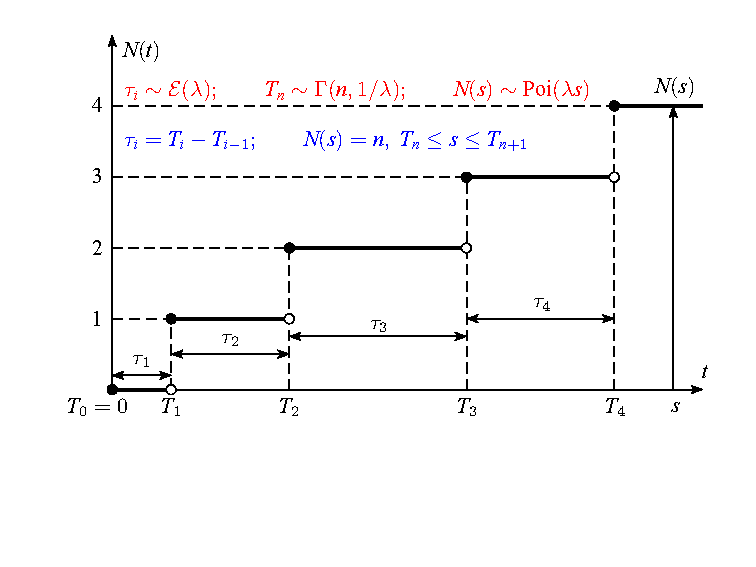
\includegraphics{fig/poisson1.pdf}
\end{frame}


\begin{frame}{两组等价关系}
\begin{center}
    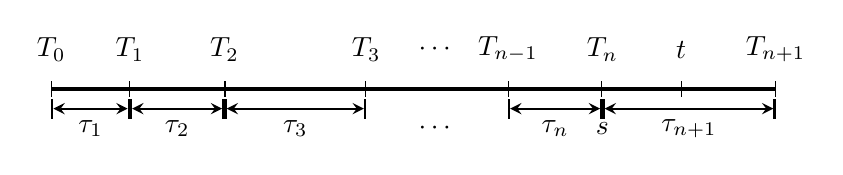
\begin{tikzpicture}[>= stealth]
        \draw (0,0)--(8,0);
        \node at (0,.5) {$T_0$};
        \node at (1,.5) {$T_1$};
        \node at (2.2,.5) {$T_2$};
        \node at (4,.5) {$T_3$};
        \node at (4.9,.5){$\cdots$};
        \node at (5.8,.5) {$T_{n-1}$};
        \node at (7,.5) {$T_{n}$};
        \node at (8,.5) {$t$};
        \node at (9.2,.5) {$T_{n+1}$};
        \draw [|<->|, thick] (0,-.25)--(1,-.25);
        \draw [|<->|, thick] (1,-.25)--(2.2,-.25);
        \draw [|<->|, thick] (2.2,-.25)--(4,-.25);
        \draw [|<->|, thick] (5.8,-.25)--(7,-.25);
        \draw [|<->|, thick] (9.2,-.25)--(7,-.25);
        \draw [very thick] (0,0)--(9.2,0);
        
        
        \node at (.5,-.5) {$\tau_1$};
        \node at (1.6,-.5) {$\tau_2$};
        \node at (3.1,-.5) {$\tau_3$};
        \node at (4.9,-.5) {$\cdots$};
        \node at (6.4,-.5) {$\tau_{n}$};
        \node at (8.1,-.5) {$\tau_{n+1}$};
        \node at (7,-.5) {$s$};
        
        \draw [|-|] (0,0)--(1,0);
        \draw [|-|] (4,0)--(2.2,0);
        \draw [|-|] (5.8,0)--(7,0);
        \draw [|-|] (9.2,0)--(8,0);
        \end{tikzpicture}
\end{center}

    \begin{enumerate}
        \item  “$t$时刻的计数不小于$n$”,等价于“计数为$n$的时刻不大于$t$时刻”,即:
    \begin{equation*}
        \{N(t)\ge n\}=\{ T_n\le t\}
    \end{equation*}
        \item	“$t$时刻的计数为$n$”,等价于“$t$时刻介于计数为$n$和$(n+1)$的时刻之间”,即:
    \begin{equation*}
        \{ N(t)= n\}=\{ T_n\le t< T_{n+1}\}
    \end{equation*}
    \end{enumerate}
\end{frame}


\begin{frame}{泊松过程的第二种定义方式}
    已知$t$时刻前的计数为$n$,即$N(t)=n$,假设在很短的时间段$[t,t+\Delta t]$内有以下概率:
\begin{align*}
\Pr[N(t+\Delta t)=n]&= 1-\lambda \Delta t+O(\Delta t)\\
\Pr[N(t+\Delta t)=n+1]&= \lambda \Delta t+O(\Delta t)\\
\Pr[N(t+\Delta t)=n+2]&= O(\Delta t)
\end{align*}
则称$N(t)$是速率/强度为$\lambda$的泊松过程,即$N(t)\sim {\rm Poi}(\lambda t)$。
\end{frame}


\subsection{泊松过程的性质}
\begin{frame}{泊松过程的性质}
    \begin{enumerate}
        \item $N(0)=0$;

        \item  $N(t+s)-N(s)\sim {\rm Poi}(\lambda t), \; N(t+0)-N(0)=N(t)\sim {\rm Poi}(\lambda t)$\\	
            即:长度相等的时间段内,事件发生个数的概率分布是相同的,也被称为{平稳增量(stationary increment)}; 
            \item  $N(t)$具有{独立增量}(independent increment),即对于$t_0<t_1<\cdots<t_n$,有:
            \[N(t_1)-N(t_0),\; N(t_2)-N(t_1),\; \ldots ,\; N(t_n)-N(t_{n-1}) \text{ 均独立。} \]
    \end{enumerate}
\end{frame}


\begin{frame}{平稳的含义}
    平稳(stationary)可以细分为严平稳(strictly stationary)和宽平稳(weakly stationary)两大类。
    
    所谓严平稳,是指一个随机过程的联合分布函数不随时间而发生改变;而宽平稳也称作协方差平稳(covariance stationary),是指一个过程的协方差不随时间而发生改变,即期望、方差和协方差不变。
    
    根据这一定义,泊松过程的增量明显满足宽平稳的基本条件。
\end{frame}



\begin{frame}{引理}
    \begin{itemize}
        \item 	$N(t+s)-N(s),\; t\ge0$是一个速率为$\lambda$的泊松过程,且与$N(r)$,$0\le r\le s$相互独立。
        \item 若对任何$0=t_0<t_1<\cdots<t_n$, $k_i$取值为正整数,且序列不减,则:
        \[\begin{split}
        \Pr&\left[N(t_n)=k_n|N(t_{n-1})=k_{n-1},\ldots, N(t_1) =k_1\right]\\
         &\qquad=\Pr\left[N(t_n)=k_n|N(t_{n-1})=k_{n-1}\right] 
        \end{split}\]
    \end{itemize}
\end{frame}


\begin{frame}{举例4}\small
    假设一个计数过程$\{N(t), t\ge 0\}$是速率为2的泊松过程,求$\Pr[N(20)-N(18)=2]$。

\begin{block}{解答}
    根据泊松过程的增量平稳性,可进行如下简化:
\[\Pr[N(20)-N(18)=2]=\Pr[N(2)=2]\]
于是此处的$t=2$, $n=2$。结合速率$\lambda=2$,可得:
\[\begin{split}
    \Pr[N(t)=n]&=\frac{(\lambda t)^n}{n!}{\rm e}^{-\lambda t}\\
    \Pr[N(2)=2]&=\frac{(2\times  2)^2}{2!}{\rm e}^{-2\times  2}=8{\rm e}^{-4}=14.65\% 
\end{split}
\]
最终可得:$$\Pr[N(20)-N(18)=2]=14.65\%$$
\end{block}

\end{frame}

\subsection{泊松过程的条件分布}
\begin{frame}{泊松过程的条件分布}
    关于泊松过程的条件分布问题,我们主要关注两点:
    \begin{enumerate}
        \item     到达时刻的条件分布;
        \item     到达次数的条件分布。
    \end{enumerate}
\end{frame}


\begin{frame}{到达时刻的条件分布举例}
    用$N(t)$表示在$t$分钟内到达商店的顾客数量。$N(t)$满足速率为$\lambda$的泊松分布,即$N(t)\sim {\rm Poi}(\lambda t)$。目前已知$N(t)=1$,假设$T_1$是第一位顾客到达的时刻,显然$T_1\le s,\; s\in(0,t)$。

求到达时刻的条件分布。

\begin{block}{思路:}
    问题转化为求解$\Pr[T_1\le s|N(t)=1]$。
\end{block}
\end{frame}


\begin{frame}{}
    由于$\{T_1\le s\}$等价于$\{N(s)\ge 1\}$,因此:
\[\Pr[T_1\le s|N(t)=1]=\Pr[N(s)\ge 1|N(t)=1]\]
需要注意的是,由于$s\le t$,在$N(t)=1$的前提条件下,$N(s)$不可能大于1,因此:
\[\begin{split}
\Pr[T_1\le s|N(t)=1]&=\Pr[N(s)= 1|N(t)=1]\\
&=\frac{\Pr[N(s)=1, N(t)=1]}{\Pr[N(t)=1]}\\
&=\frac{\Pr[N(s)=1, N(t)-N(s)=0]}{\Pr[N(t)=1]}\\
&=\frac{\Pr[N(s)=1]\cdot \Pr[N(t-s)=0]}{\Pr[N(t)=1]}\\
&=\frac{\lambda s{\rm e}^{-\lambda s}\cdot {\rm e}^{-\lambda(t-s)}}{\lambda t{\rm e}^{-\lambda t}}=\frac{s}{t}
\end{split}\]
\end{frame}


\begin{frame}{到达时刻的条件分布结论}
    最终得到的条件分布函数和条件密度函数如下:
\begin{enumerate}
\item 条件概率分布函数:
\[F(s)=\Pr[T_1\le s|N(t)=1]=\Pr[N(s)\ge 1|N(t)=1]=\frac{s}{t}\]
\item 	条件概率密度函数:
\[f(s)=\frac{\dif F(s)}{\dif s}=\frac{1}{t},\qquad s\in(0,t) \]
\end{enumerate}
因此在$t$时刻之前有一个顾客到达的条件下,其到达的时刻$T_1$服从$[0,t]$上的{均匀分布}(uniform distribution)。 
\end{frame}


\begin{frame}{问题引申}\small
    在$N(t)=2$的条件下,到达时刻的条件分布及其概率密度分别为多少?
\begin{block}{思路:}
     取$s_1<s_2$,使得$s_1\ge T_1,\; s_2\ge T_2$,构造条件分布$F(s_1,s_2)$,表达式如下:
\[F(s_1,s_2)=\Pr\big(T_1\le s_1,T_2\le s_2|N(t)=2\big)\]
\end{block}
   
\begin{center}
    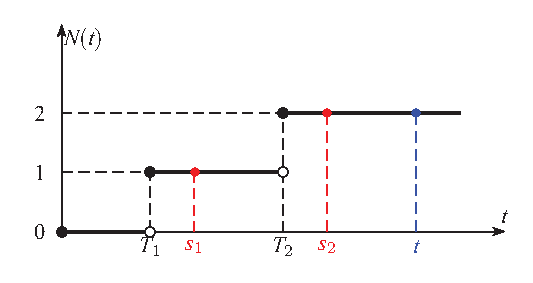
\includegraphics{fig/poisson5.eps}
\end{center}
\end{frame}



\begin{frame}{推导过程}\small
    \[\begin{split}
        F(s_1,s_2)&=\Pr\big[T_1\le s_1,T_2\le s_2|N(t)=2\big]\\&=\Pr\big[N(s_1)=1,N(s_2)=2|N(t)=2\big]\\
        &=\frac{\Pr[N(s_1)=1,N(s_2)=2,N(t)=2]}{\Pr[N(t)=2]}\\
        &=\frac{\Pr[N(s_1)=1]\cdot \Pr[N(s_2)-N(s_1)=1]\cdot \Pr[N(t)-N(s_2)=0]}{\Pr[N(t)=2]}\\
        \end{split}\]
        \[\begin{split}
        &=\frac{\Pr[N(s_1)=1]\cdot \Pr[N(s_2-s_1)=1]\cdot \Pr[N(t-s_2)=0]}{\Pr[N(t)=2]}\\
        &=\frac{\lambda s_1{\rm e}^{-\lambda s_1}\cdot \lambda (s_2-s_1){\rm e}^{-\lambda (s_2-s_1)}\cdot {\rm e}^{-\lambda(t-s_2)}}{\frac{1}{2}(\lambda t)^2{\rm e}^{-\lambda t}}\\
        &=\frac{2s_1(s_2-s_1)}{t^2}=\frac{2s_1s_2-2s^2_1}{t^2}
        \end{split}\]
\end{frame}


\begin{frame}{条件分布和条件概率密度}
    条件分布:
    \[F(s_1,s_2)=\frac{2s_1s_2-2s^2_1}{t^2}\]
    条件概率密度:\[f(s_1,s_2)=\frac{\partial^2 F(s_1s_2)}{\partial s_1\partial s_2}=\frac{2}{t^2} \]


    按照类似的方法可以得到在条件$N(t)=n>0$下, $(T_1,T_2,\ldots,T_n)$的联合密度函数如下:
\[f(s_1,s_2,\ldots,s_n)=\frac{n!}{t^n}\]
\end{frame}


\begin{frame}{到达次数的条件分布}
    如果$s<t$,且$0\le m\le n$,那么
\[\Pr[N(s)=m|N(t)=n]={n \choose m}\left(\frac{s}{t}\right)^m\left(1-\frac{s}{t}\right)^{n-m} \]
即在给定$N(t)=n$时,$N(s)$的条件分布是二项分布$B(n,s/t)$。
\end{frame}


\begin{frame}{到达次数的条件分布(cont.)}
    由于$s<t$,且$0\le m\le n$,因此:
\[\begin{split}
\Pr[N(s)=m|N(t)=n]&=\frac{\Pr[N(s)=m,N(t)=n]}{\Pr[N(t)=n]}\\
&=\frac{\Pr[N(s)=m, N(t-s)=n-m]}{\Pr[N(t)=n]}\\
&=\frac{\Pr[N(s)=m]\cdot\Pr[N(t-s)=n-m]}{\Pr[N(t)=n]}\\
&=\frac{\frac{(\lambda s)^m}{m!}{\rm e}^{-\lambda s}\cdot \frac{[\lambda (t-s)]^{n-m}}{(n-m)!}{\rm e}^{-\lambda (t-s)}}{\frac{(\lambda t)^n}{n!}{\rm e}^{-\lambda t}}\\&=\frac{n!}{m!(n-m)!}\cdot \frac{s^m\cdot (t-s)^{n-m}}{t^n}\\
&={n \choose m} \cdot \frac{s^m\cdot (t-s)^{n-m}}{t^m\cdot t^{n-m}}={n \choose m} \cdot \left(\frac{s}{t} \right)^m \left(\frac{t-s}{t} \right) ^{n-m} 
\end{split}\]
\end{frame}


\begin{frame}{到达次数的条件分布(cont.)}
\[\Pr[N(s)=m|N(t)=n]={n \choose m} \cdot \left(\frac{s}{t} \right)^m \left(\frac{t-s}{t} \right) ^{n-m} \]
    根据最终的结果不难看出:到达次数的条件分布服从$n$次试验中成功次数为$m$、成功概率为$s/t$的二项分布,即$B\left(n,s/t\right)$。
\end{frame}


\begin{frame}{注意}
    如果将条件概率公式当中的条件和结果颠倒,得到的结果是泊松分布,具体计算过程如下:
\[\begin{split}
\Pr[N(t)=n|N(s)=m]&=\frac{\Pr[N(t)=n,N(s)=m]}{\Pr[N(s)=m]}\\
&=\frac{\Pr[N(s)=m]\cdot\Pr[N(t-s)=n-m]}{\Pr[N(s)=m]}\\
&=\Pr[N(t-s)=n-m]\\
&=\frac{[\lambda(t-s)]^{n-m}}{(n-m)!}{\rm e}^{-\lambda(t-s)} 
\end{split}\]
\end{frame}


\subsection{泊松过程的变换}


\begin{frame}{泊松过程的变换}
    泊松过程的变换分为两大类:一类是稀释(thinning),即某一个泊松过程可以拆分成若干个独立的泊松过程;另一类是叠加(superposition),即若干个独立的泊松过程可以合成一个泊松过程。
\end{frame}


\begin{frame}{泊松过程的稀释}
设$N(t)$是速率为$\lambda$的泊松过程[即$N(t)\sim {\rm Poi}(\lambda t)$],表示到$t$时刻记录的事件个数。假设其中每个事件被记录的概率为$p$,且事件是否被记录是独立的。若被记录的事件记为$N_1(t),\; t\ge 0$,则:
$N_1(t)\sim {\rm Poi}(p\lambda  t)$

\begin{center}
    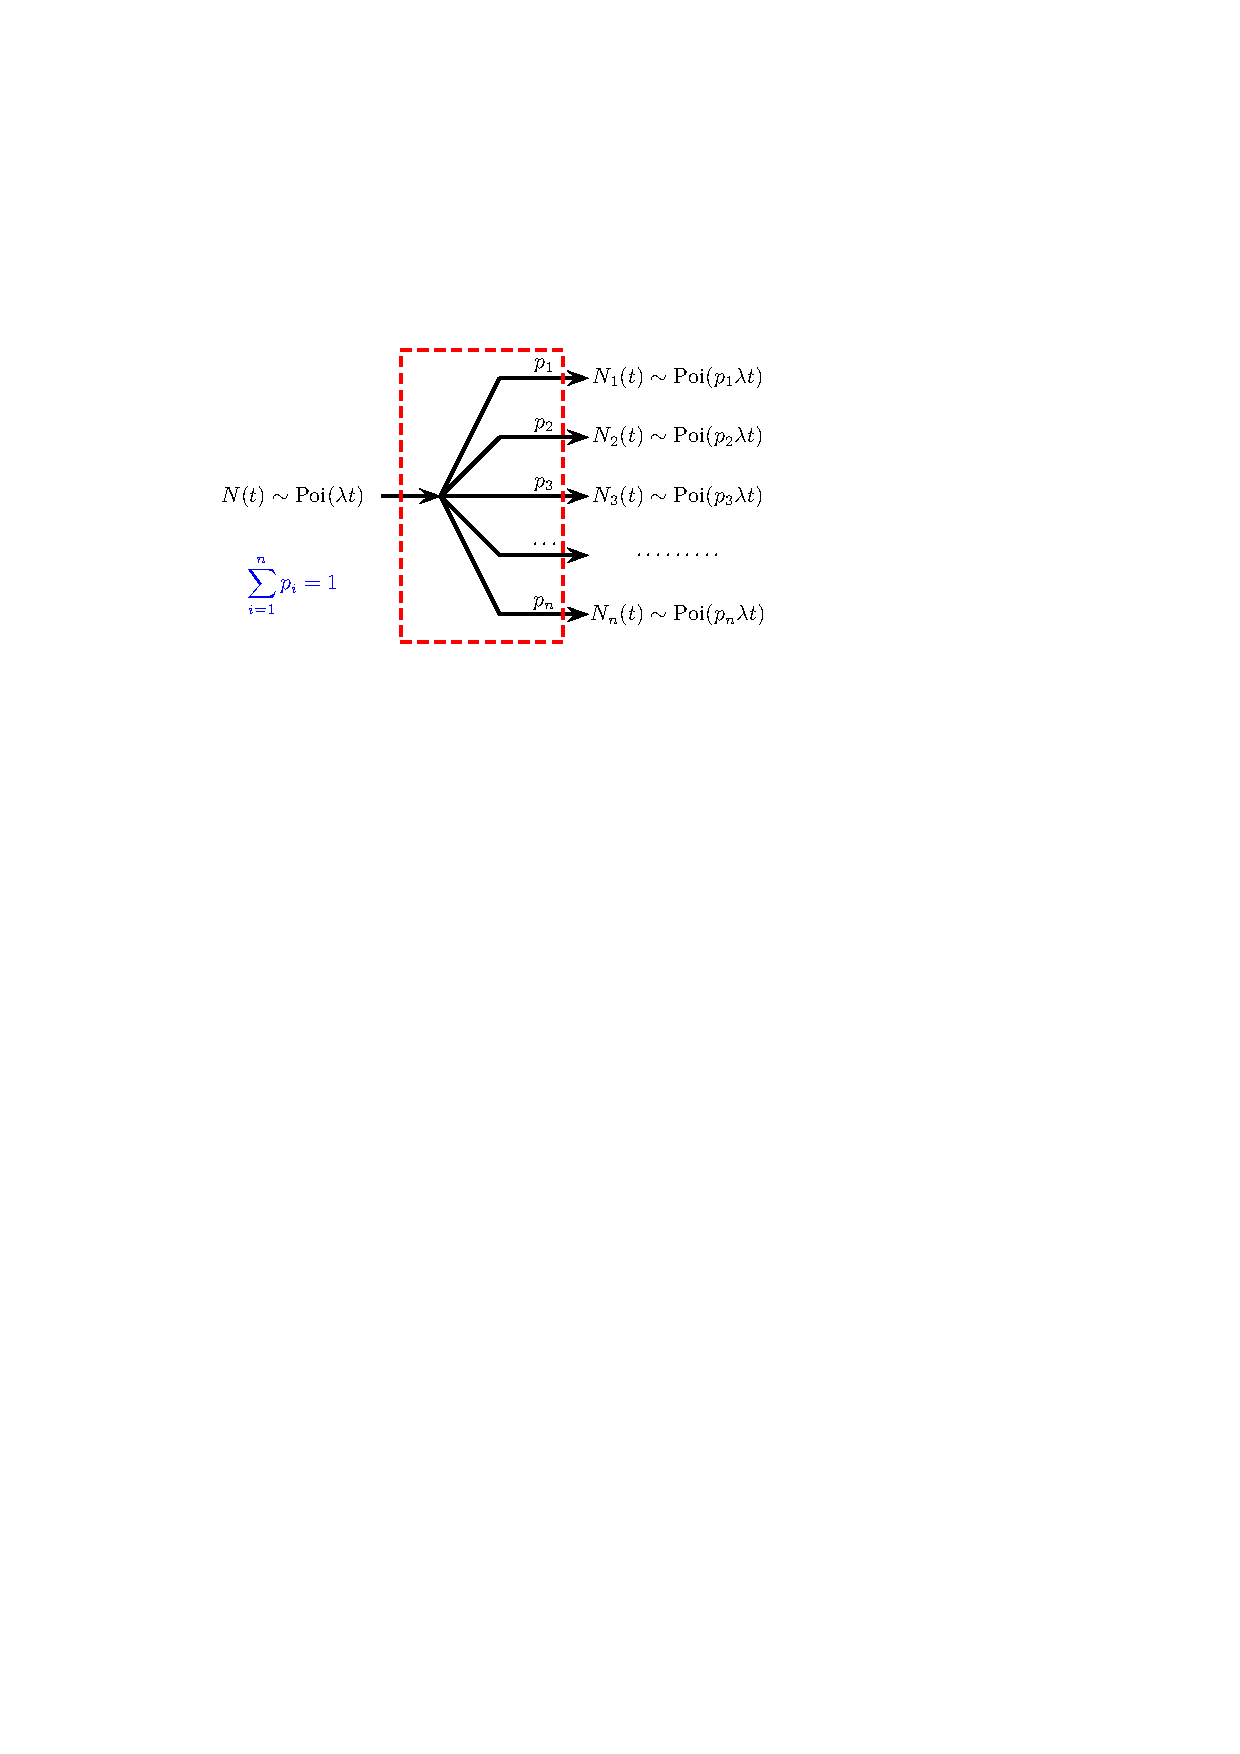
\includegraphics[scale=0.85]{fig/poisson2.pdf}
\end{center}
\end{frame}



\begin{frame}{推导过程}
    根据全概率公式,可得:
\[ \begin{split}
\Pr[N_1(t)=n]&=\sum_{m=0}^{\infty}{\Pr[N_1(t)=n|N(t)=m+n]}\cdot \Pr[N(t)=m+n]\\
&=\sum_{m=0}^{\infty}{{m+n \choose n}p^n(1-p)^m}\cdot {\rm e}^{-\lambda t}\frac{(\lambda t)^{m+n}}{(m+n)!}\\
&=\sum_{m=0}^{\infty}{\frac{{(m+n)!}}{m!\; n!}	p^n(1-p)^m}\cdot {\rm e}^{-\lambda t}\frac{(\lambda t)^{m+n}}{{(m+n)!}}\\
\end{split} \]

$\Pr[N_1(t)=n|N(t)=m+n]$表示$(m+n)$个事件当中,被记录的事件有$n$个的概率。由于事件是否被记录是独立的,因此这里可看作
成功概率为$p$的二项分布,相应的概率就是:
\[\Pr[N_1(t)=n|N(t)=m+n]={m+n \choose n}p^n(1-p)^m\]
\end{frame}



\begin{frame}{推导过程(cont.)}
    根据${\rm e}^x=\displaystyle\sum_{n=0}^{\infty}\frac{x^n}{n!}$,可得:
\[\begin{split}
\Pr[N_1(t)=n]&= {\rm e}^{-\lambda t}\sum_{m=0}^{\infty}\frac{(1-p)^m(\lambda t)^m}{m!}\cdot\frac{p^n(\lambda t)^n}{n!}\\
\end{split} \]
\[\begin{split} 
&={\rm e}^{-\lambda t}\frac{(p\lambda t)^n}{n!}\sum_{m=0}^{\infty}\frac{[(1-p)\lambda t]^m}{m!}\\
&={\rm e}^{-\lambda t}\frac{(p\lambda t)^n}{n!}\cdot {\rm e}^{(1-p)\lambda t}={\rm e}^{-p\lambda t}\frac{(p\lambda t)^n}{n!}\\
\end{split} \]
因此:$$N_1(t)\sim {\rm Poi}(p\lambda  t)$$
\end{frame}


\begin{frame}{泊松过程的叠加}
假设$N_1(t),\ldots, N_k(t)$是独立的泊松过程,速率分别为$\lambda_1,\ldots,\lambda_k$,则$N_1(t)+\cdots+N_k(t)$是一个泊松过程,并且速率为$\lambda_1+\cdots+\lambda_k$。
\begin{center}
    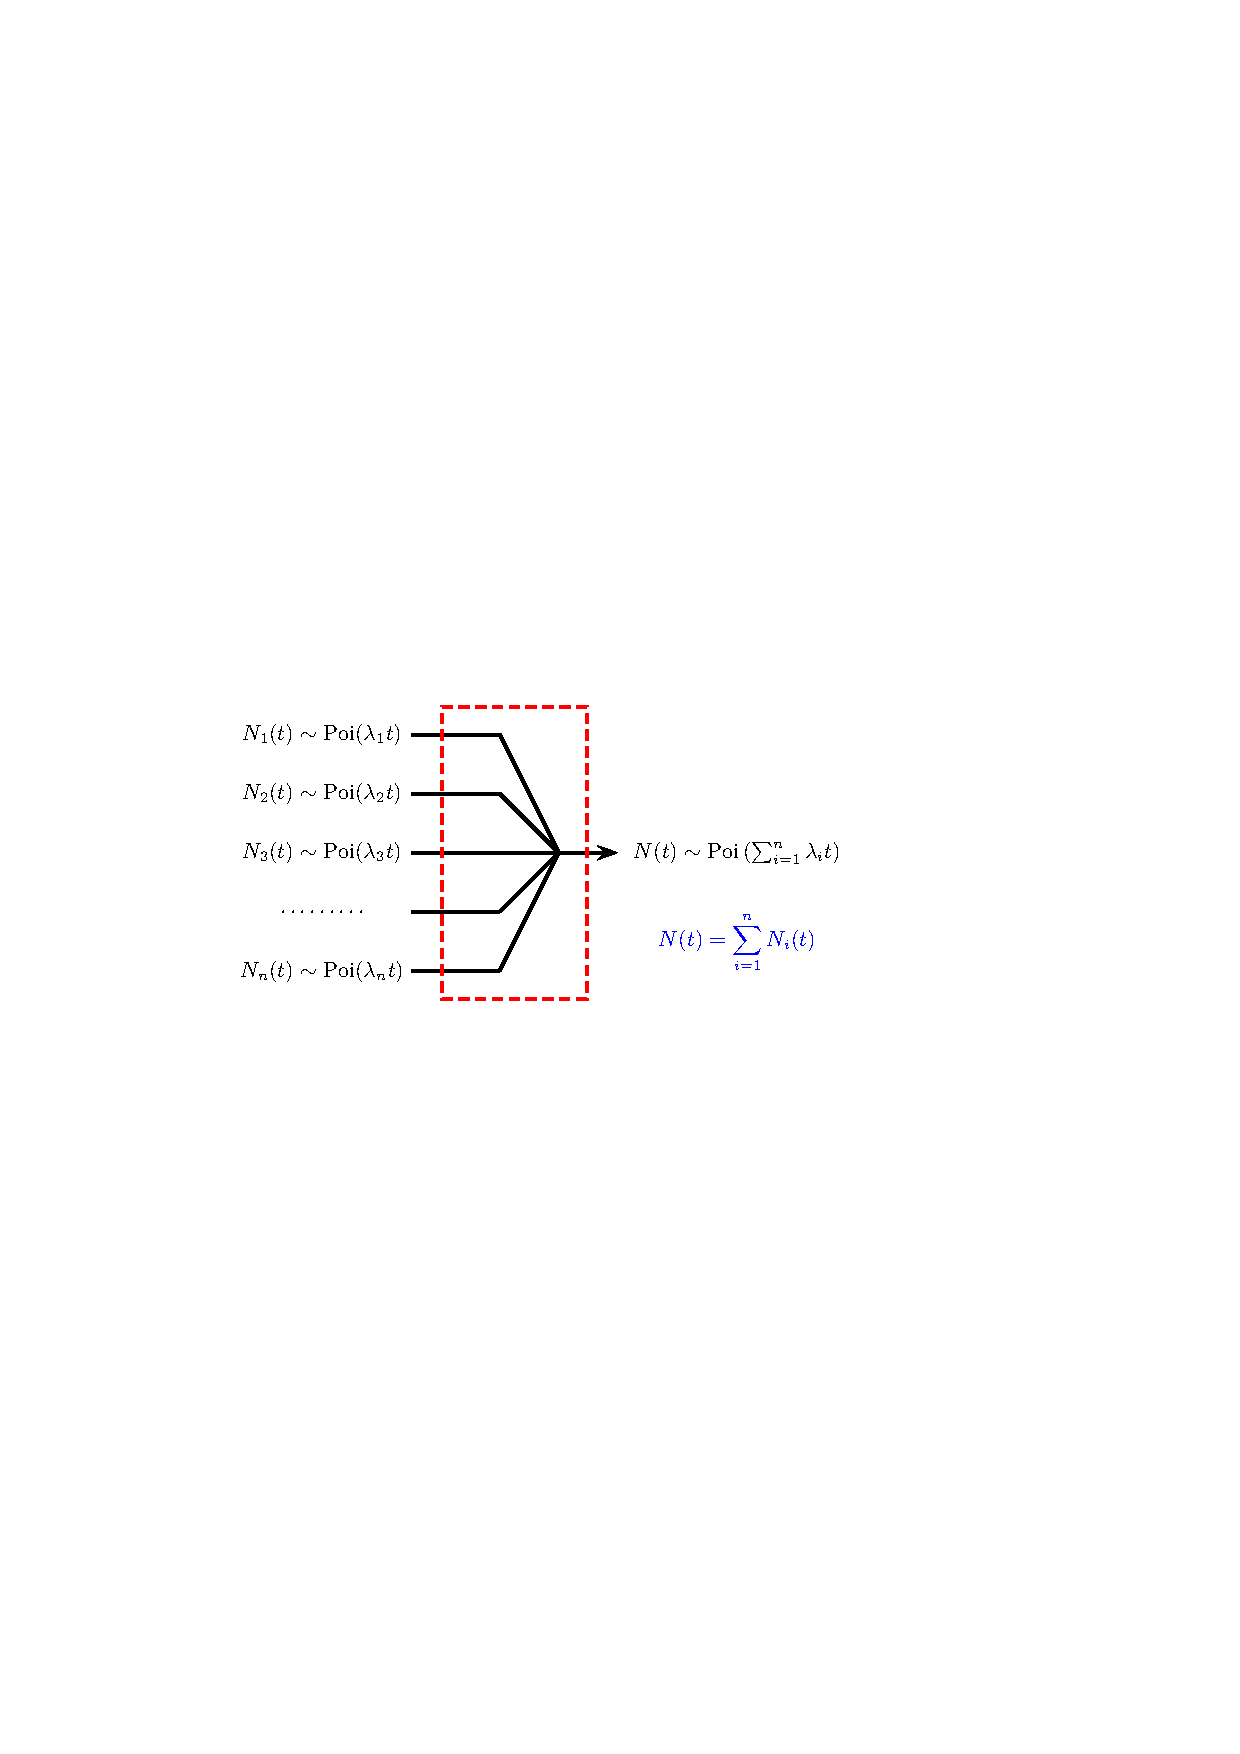
\includegraphics[scale=0.85]{fig/poisson3.pdf}
\end{center}
\end{frame}

\section{泊松过程的拓展}
\begin{frame}{泊松过程的拓展}
    前面所介绍的泊松过程,从严格意义上讲是一种特殊的齐次泊松过程。在现实应用中需要对其进行一定的拓展。具有代表性的拓展有两类:
    \begin{itemize}
        \item     非齐次泊松过程;
        \item     复合泊松过程。
    \end{itemize}

\end{frame}

\subsection{非齐次泊松过程}
\begin{frame}{非齐次泊松过程}
    满足以下条件的计数过程$\{N(t): t\ge0 \}$就是强度函数为$\lambda(t)$的非齐次泊松过程(nonhomogeneous Poisson process)。
	\begin{enumerate}[\quad\;(1)]
		\item $N(0)=0$;
		\item $N(t)$具有独立增量性;
		\item $ 
		\E[N(r)-N(s)]=\displaystyle\int_{s}^{r} \lambda(t) \dif t,\quad  
		N(r)-N(s) \sim \text{Poi}\left(\displaystyle\int_{s}^{r} \lambda(t) \dif t\right)$。
    \end{enumerate}
    
    \begin{block}{注意:}
        此时的时间间隔$\tau_1,\tau_2,\ldots$不再服从指数分布,并且不满足独立性条件。当$\lambda(t)=\lambda$时,强度/速率不随时间而发生改变,此时便是我们所熟悉的(齐次)泊松过程。 
    \end{block}
\end{frame}


\begin{frame}{非齐次泊松过程的性质}
    非齐次泊松过程在$t$时刻计数为$n$的概率如下:
    \[\Pr[N(t)=n]=p_n(t)=\frac{[m(0,t)]^n}{n!}\exp\left[-m(0,t) \right] \]
    其中:\[m(s,t)= \int^t_s \lambda(t')\dif t' \]
  
    非齐次泊松过程的期望和方差:
\begin{equation*}
\E[N(t)]=\Var[N(t)]=m(0,t)= \int^t_0 \lambda(t')\dif t'
\end{equation*}
\end{frame}


\begin{frame}{举例5}
    设$\{X(t), t\ge0\}$是一个强度函数为$\lambda(t)=\displaystyle\frac{1}{2}(1+\cos\omega t)$的非齐次泊松过程,其中$\omega\ne 0$。

求$\E[X(t)]$和$\Var[X(t)]$。

\begin{block}{}
    \[\begin{split}
        \E[X(t)]=\Var[X(t)]&=\int^t_0 \lambda(t') \dif t'=\int^t_0 \frac{1}{2}(1+\cos\omega t')\dif t'\\
        &=\frac{1}{2}\left.\left(t'+\frac{1}{\omega}\sin \omega t'\right)\right|^{t'=t}_{t'=0}\\
        &=\frac{1}{2}\left(t+\frac{1}{\omega}\sin \omega t\right)
        \end{split} \]
\end{block}
\end{frame}


\begin{frame}{举例6}
    设某路公共汽车从早晨5时到晚上21时有车发出,乘客流量如下:
5时按平均乘客为200人/小时计算;5时至8时乘客平均到达率线性增加,8时
到达率为1400人/小时;8时至18时保持平均到达率不变;18时至21时到达率以
1400人/小时线性下降,到21时为200人/小时。假定乘客数在不重叠的时间间隔
内是相互独立的。

求12时至14时有2000人来站乘车的概率,并求出这两个小时内
来站乘车的人数的期望值。

\end{frame}



\begin{frame}{举例6(cont.)}\small
    \begin{block}{思路:}
        将刚开始的早晨5时记为时刻$t=0$,其他的时间以此类推,最终21时记为时刻$t=16$。由此可以得到乘客到达率的函数$\lambda(t)$如下:
    \[\lambda(t)=\begin{cases}
    200+400t, & t\in [0,3]\\
    1400, & t\in [3,13]\\
    1400-400(t-13), & t\in [13,16]\\
    \end{cases} \]
    \end{block}
    \begin{center}
		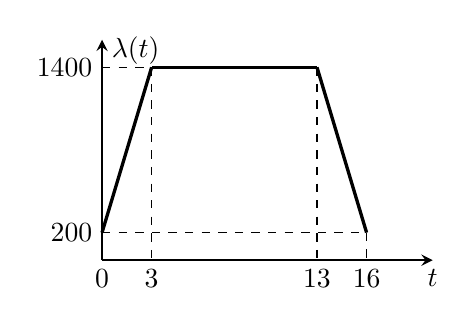
\begin{tikzpicture}[>=stealth,scale=.7]
		\draw [->, thick](0,0)--(6,0);
		\draw [->, thick](0,0)--(0,4);
		\draw [dashed] (0,0.5)--(4.8,0.5);
		\draw  [dashed](0,3.5)--(0.9,3.5);
		
		\draw [very thick] (0,0.5)--(0.9,3.5);
		\draw [very thick] (3.9,3.5)--(0.9,3.5);
		\draw [very thick] (4.8,0.5)--(3.9,3.5);
		\draw  [dashed] (0.9,3.5)--(0.9,0);
		\draw  [dashed] (3.9,3.5)--(3.9,0);
		\draw  [dashed] (4.8,0.5)--(4.8,0);
		
		\node at (6,0) [below] {$t$};
		\node at (0.9,0) [below] {3};
		\node at (3.9,0)[below]  {13};
		\node at (4.8,0) [below] {16};
		\node at (0,0) [below] {0};
		\node at (0,0.5)[left]  {200};
		\node at (0,3.5)[left]  {1400};
		\node at (0,3.8)[right]  {$\lambda(t)$};
		
		\end{tikzpicture}
		\end{center}
\end{frame}


\begin{frame}{举例6(cont.)}
    所要求的时间段应当为$t\in[7,9]$,相应地:
    \[m(7,9)=\int^9_7 \lambda(t)\dif t=\int^9_7 1400 \dif t=1400\times(9-7)=2800\text{(人)} \]

    在12时到14时有2000名乘客到达的概率为:
    \[\Pr[N(9)-N(7)=2000]={\rm e}^{-m(7,9)}\frac{[m(7,9)]^n}{n!}={\rm e}^{-2800}\frac{2800^{2000}}{2000!} \]
    相应地,这段时间内乘客数的期望值即为:
    $$m(7,9)=2800\text{(人)}$$ 
\end{frame}

\subsection{复合泊松过程}
\begin{frame}{复合泊松过程}
    满足以下条件的$\{S(t):t\ge0\}$就是复合泊松过程(compound Poisson process):
\[S(t)=Y_1+Y_2+\cdots +Y_{N(t)}=\sum^{N(t)}_{i=1}Y_i \]
其中,$\{N(t):t\ge0\}$是比率为$\lambda$的泊松过程;$\{Y_i:i\ge1\}$是独立同分布的随机变量,
且$\{Y_i\}$的分布函数与泊松过程$\{N(t):t\ge0\}$是 独立的。	
\end{frame}


\begin{frame}{复合泊松过程与泊松过程}
    先前的泊松过程可看作复合泊松过程的特殊情形(此时$Y_i\equiv 1$)
 \begin{center}
    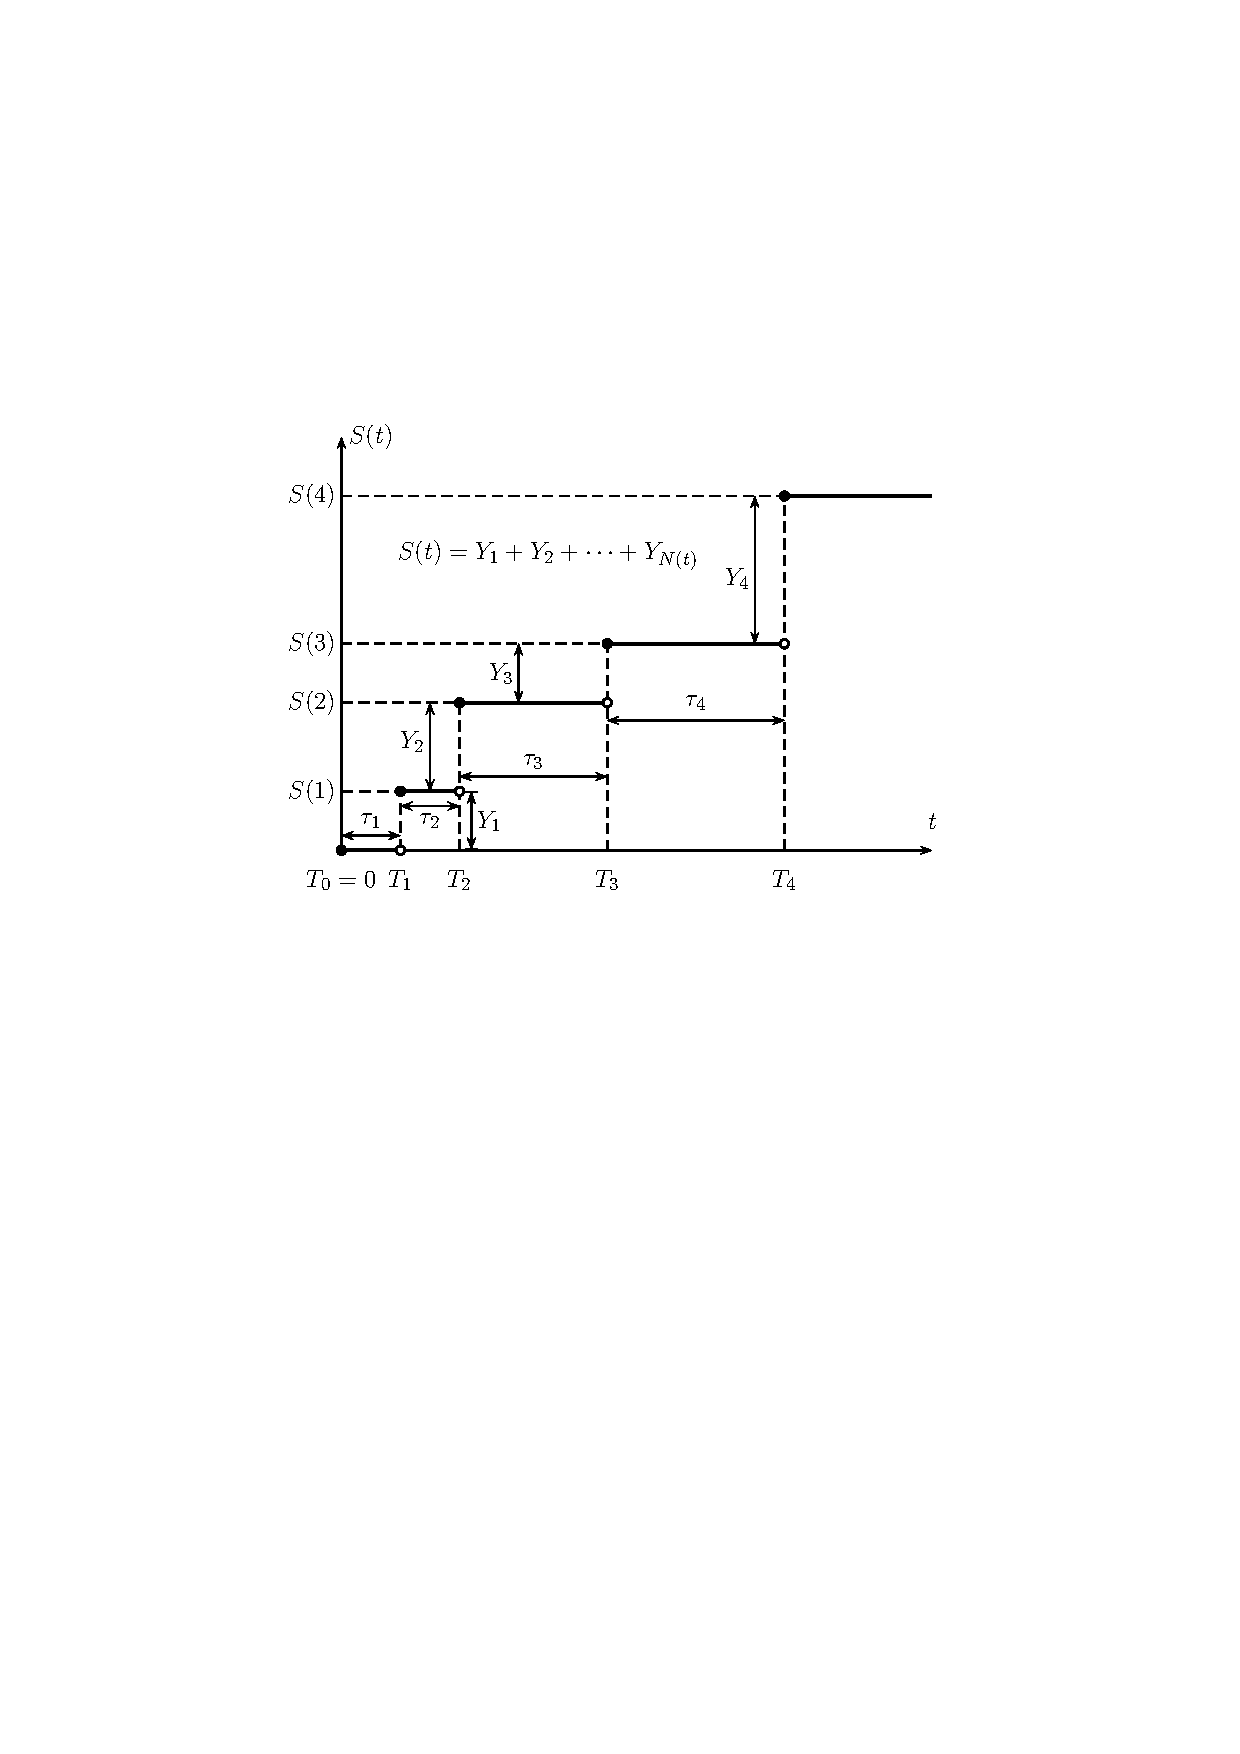
\includegraphics[scale=.82]{fig/poisson_comp.pdf}
 \end{center}
\end{frame}


\begin{frame}{复合泊松过程举例1}
    假设$N(t)$是在时间段$[0,t]$内到达某商店的人数,并且$\{N(t), t\ge 0\}$是泊松过程。假设$Y_k$是到达商店的顾客$k$消费的金额,如果假设$\{Y_k\}, \; k=1,2,\ldots,N(t)$是独立同分布的随机变量序列,并且与$\{N(t)\}$独立,
那么商店在时间段$[0,t]$内的总营业额$X(t)$就是:
\[X(t)=\sum^{N(t)}_{k=1}Y_k, \qquad t \ge 0 \]
这里的$\{X(t), \; t\ge 0\}$就是一个复合泊松过程。
\end{frame}


\begin{frame}{复合泊松过程举例2}
    在股票市场上,假设$N(t)$是某股票在时间段$[0,t]$内跳空上涨或下跌的次数,并且$\{N(t), t\ge 0\}$是泊松过程。假设$Y_k$是股价第$k$次跳跃的幅度,股价的跳跃幅度$\{Y_k\}, \; k=1,2,\ldots,N(t)$是独立同分布的随机变量序列,并且与$\{N(t)\}$独立。

那么在时间段$[0,t]$内,该股票价格总的跳跃幅度$X(t)$就是:
\[X(t)=\sum^{N(t)}_{k=1}Y_k, \qquad t\ge 0 \]
这里的$\{X(t), \; t\ge 0\}$也是一个复合泊松过程。
\end{frame}


\begin{frame}{随机和}
    \begin{block}{定理:}
        假设$Y_1,Y_2,\ldots$表示独立同分布的随机变量,并且均值为$\mu$、方差为$\sigma^2$,已知$S(t)=Y_1+Y_2+\cdots+Y_{N(t)}$,其中$\{N(t):t\ge 0\}$是速率为$\lambda$的泊松过程。则$S(t)$的均值和方差分别如下:
        \[\E[S(t)]=\mu\lambda t,\quad \Var[S(t)]=\lambda t(\sigma^2+\mu^2) \]
    \end{block}
\end{frame}



\begin{frame}{随机和的期望}
    由于$\{N(t)\}$是速率为$\lambda$的泊松过程,因此:
	\[\E[N(t)]=\Var[N(t)]=\lambda t \]
首先求出$\E[S(t)]$,具体如下:
\[\begin{split}
\E[S(t)]&= \sum^{\infty}_{n=0}\E[S(t)|N(t)=n]\cdot \Pr[N(t)=n]\\
&=\sum^{\infty}_{n=0} n\mu\cdot \frac{(\lambda t)^n}{n!}{\rm e}^{-\lambda t}\\
&=\mu \lambda t\cdot {\rm e}^{-\lambda t}\sum^{\infty}_{n=0} \frac{(\lambda t)^{n-1}}{(n-1)!}=\mu \lambda t\cdot {\rm e}^{-\lambda t}\sum^{\infty}_{k=0} \frac{(\lambda t)^k}{k!}\\
&=\mu \lambda t\cdot {\rm e}^{-\lambda t}\cdot {\rm e}^{\lambda t}=\mu \lambda t
\end{split} \]
\end{frame}


\begin{frame}{随机和的二阶矩}
    接下来求出$\E[S^2(t)]$,具体如下:
    \[\begin{split}
    \E[S^2(t)]&= \sum^{\infty}_{n=0}\E[S^2(t)|N(t)=n]\cdot \Pr[N(t)=n]\\
    &=  \sum^{\infty}_{n=0}(n^2\mu^2+n\sigma^2)\cdot \frac{(\lambda t)^n}{n!}{\rm e}^{-\lambda t}\\
        &=\mu^2  \sum^{\infty}_{n=0}  n^2\cdot\frac{(\lambda t)^n}{n!}{\rm e}^{-\lambda t}+\sigma^2 \sum^{\infty}_{n=0}  n\cdot\frac{(\lambda t)^n}{n!}{\rm e}^{-\lambda t}  \\
        &=\mu^2  \sum^{\infty}_{n=0}  n^2\cdot \Pr[N(t)=n]   +\sigma^2 \sum^{\infty}_{n=0}  n \cdot \Pr[N(t)=n]   \\
    &=\mu^2 \E[N^2(t)]+\sigma^2 \E[N(t)]
    \end{split} \]
\end{frame}


\begin{frame}{随机和的方差}
    最后求出$\Var[S(t)]$:
    \[\begin{split}
    \Var[S(t)]&= \E\left[S^2(t)\right]-\left[\E S(t) \right]^2\\
    &=\mu^2 \E\left[N^2(t) \right]+\sigma^2 \E[N(t)]-\mu^2 \left\{\E[N(t)] \right\}^2\\
    &=\sigma^2 \E[N(t)]+\mu^2\left\{ \E\left[N^2(t)\right]-\left\{\E[N(t)] \right\}^2 \right\}
    \\
    &=\sigma^2 \E[N(t)]+\mu^2 \Var[N(t)]\\
    &=\lambda t(\sigma^2+\mu^2)
    \end{split} \]  
\end{frame}





\end{document}
